\subsection{Analysis on Salsa20’s PRG}
\begin{frame}
\frametitle{Analysis on Salsa20's PRG}

\setlength{\columnsep}{10pt}
\begin{multicols}{2}
\setlength{\leftmargin}{1pt}

{\begin{itemize}
    \item \small{Line $1$, shows how, $HD(input_{original}, \ input_{next})$ is roughly equal to $1$ per flipped bits.}
    \item \small{Line $2$, is the expected value for random inputs and outputs.}
    \item \small{Line $0$, seems to be no correlation or pattern between the amounts of bits flipped in the $input(n)$ and the $HD$ between the two values.}
\end{itemize}}

\columnbreak
\setlength{\rightmargin}{0pt}
\begin{figure}
    \centering
    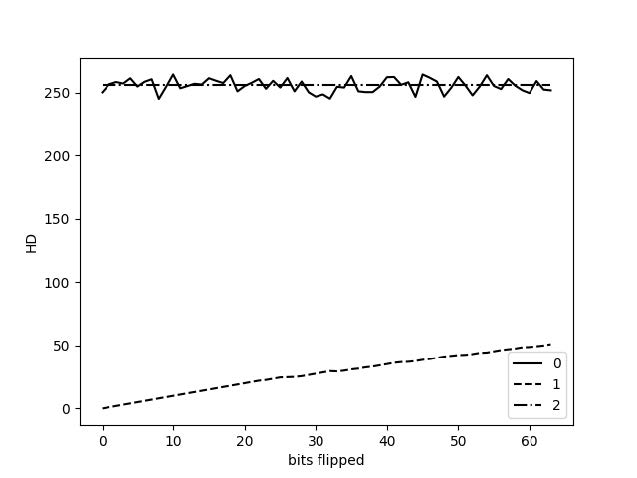
\includegraphics[scale=0.55]{fig3.jpg}
    \caption{Averaging of effects on the $PRG$ output when bits are 
flipped in key}
\end{figure}

\end{multicols}

\end{frame}